
        \documentclass[tikz, border=10pt]{standalone}
        \usepackage{tikz}
        \usetikzlibrary{arrows.meta, shapes, positioning}
        \usepackage{xcolor}
        \definecolor{brightmaroon}{RGB}{195,33,72}
        \definecolor{cyan}{RGB}{0,255,255}
        \definecolor{skyblue}{RGB}{135,206,235}
        \begin{document}
        		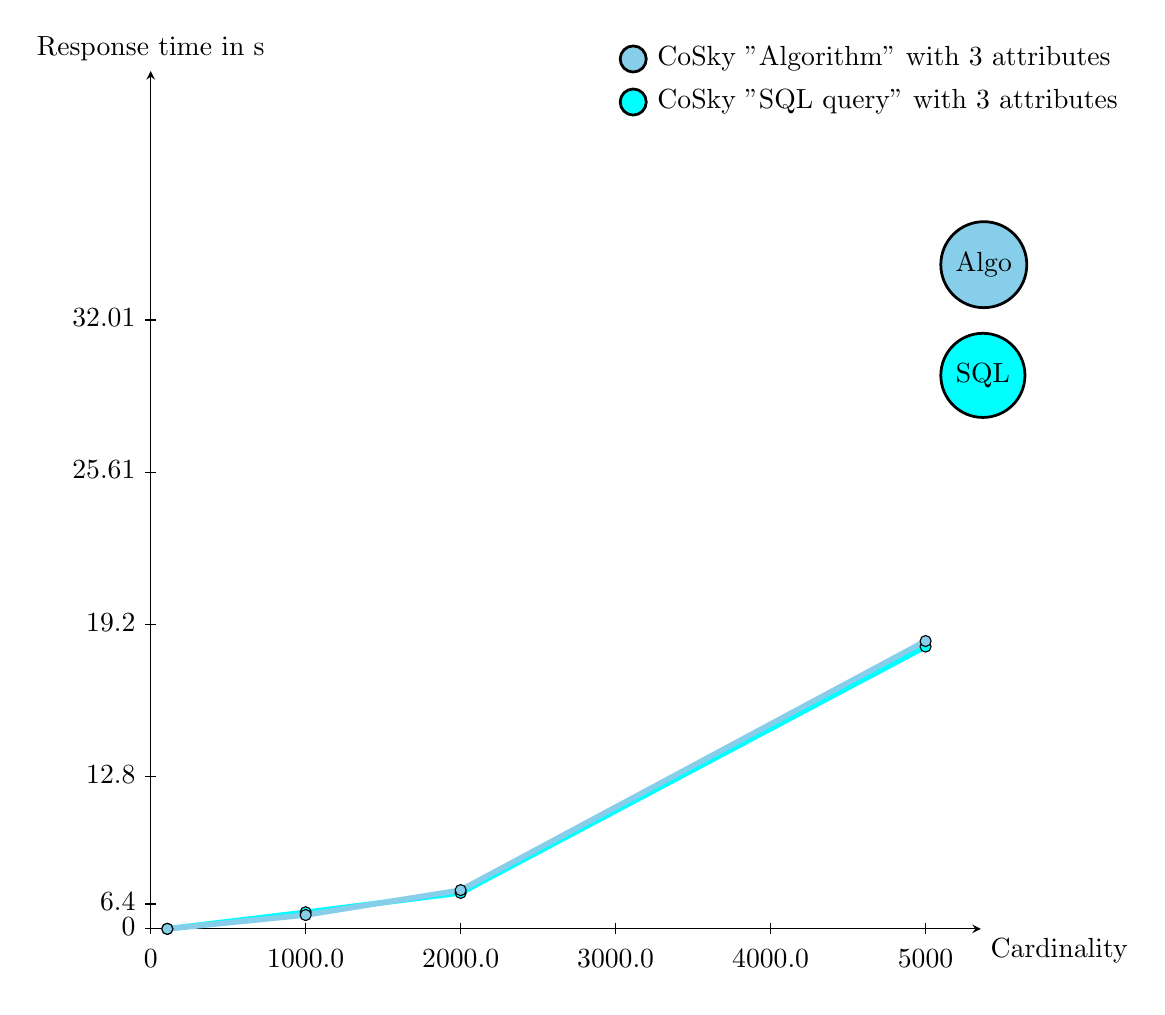
\begin{tikzpicture}[
        			line join=bevel,
        			bigcyannode/.style={shape=circle, fill=cyan, draw=black, line width=1pt},
        			bigskybluenode/.style={shape=circle, fill=skyblue, draw=black, line width=1pt}
        			]

        			%% Draws
        			\draw[-stealth] (0pt, 0pt) -- (300pt, 0pt) node[anchor=north west] {Cardinality};
        			\draw[-stealth] (0pt, 0pt) -- (0pt, 310pt) node[anchor=south] {Response time in s};
% Axis Graduation
                            \foreach \x/\xtext in {0pt/$0$, 56pt/$1000.0$, 112pt/$2000.0$, 168pt/$3000.0$, 224pt/$4000.0$, 280pt/$5000$} {
                                \draw (\x, 2pt) -- (\x, -2pt) node[below] {\xtext\strut};
                            }
                            \foreach \y/\ytext in {0pt/$0$, 9pt/$6.4$, 55pt/$12.8$, 110pt/$19.2$, 165pt/$25.61$, 220pt/$32.01$} {
                                \draw (2pt, \y) -- (-2pt, \y) node[left] {\ytext\strut};
                            }
                
\draw[cyan, line width=2pt](6pt, 0pt) -- (56pt, 6pt) -- (112pt, 13pt) -- (280pt, 102pt);

\draw[skyblue, line width=2pt](6pt, 0pt) -- (56pt, 5pt) -- (112pt, 14pt) -- (280pt, 104pt);

\filldraw[color=black, fill=cyan] (6pt, 0pt) circle (2pt);
\filldraw[color=black, fill=cyan] (56pt, 6pt) circle (2pt);
\filldraw[color=black, fill=cyan] (112pt, 13pt) circle (2pt);
\filldraw[color=black, fill=cyan] (280pt, 102pt) circle (2pt);

\filldraw[color=black, fill=skyblue] (6pt, 0pt) circle (2pt);
\filldraw[color=black, fill=skyblue] (56pt, 5pt) circle (2pt);
\filldraw[color=black, fill=skyblue] (112pt, 14pt) circle (2pt);
\filldraw[color=black, fill=skyblue] (280pt, 104pt) circle (2pt);


                %% Caption
                \matrix [below left] at (current bounding box.north east) {
                \node [bigskybluenode, label=right:CoSky "Algorithm" with 3 attributes] {}; \\
                \node [bigcyannode, label=right:CoSky "SQL query" with 3 attributes] {}; \\
                };
                
        \node[bigskybluenode, right=5pt] at (280pt,240pt) {Algo};
        \node[bigcyannode, right=5pt] at (280pt,200pt) {SQL};
        \end{tikzpicture}
        
                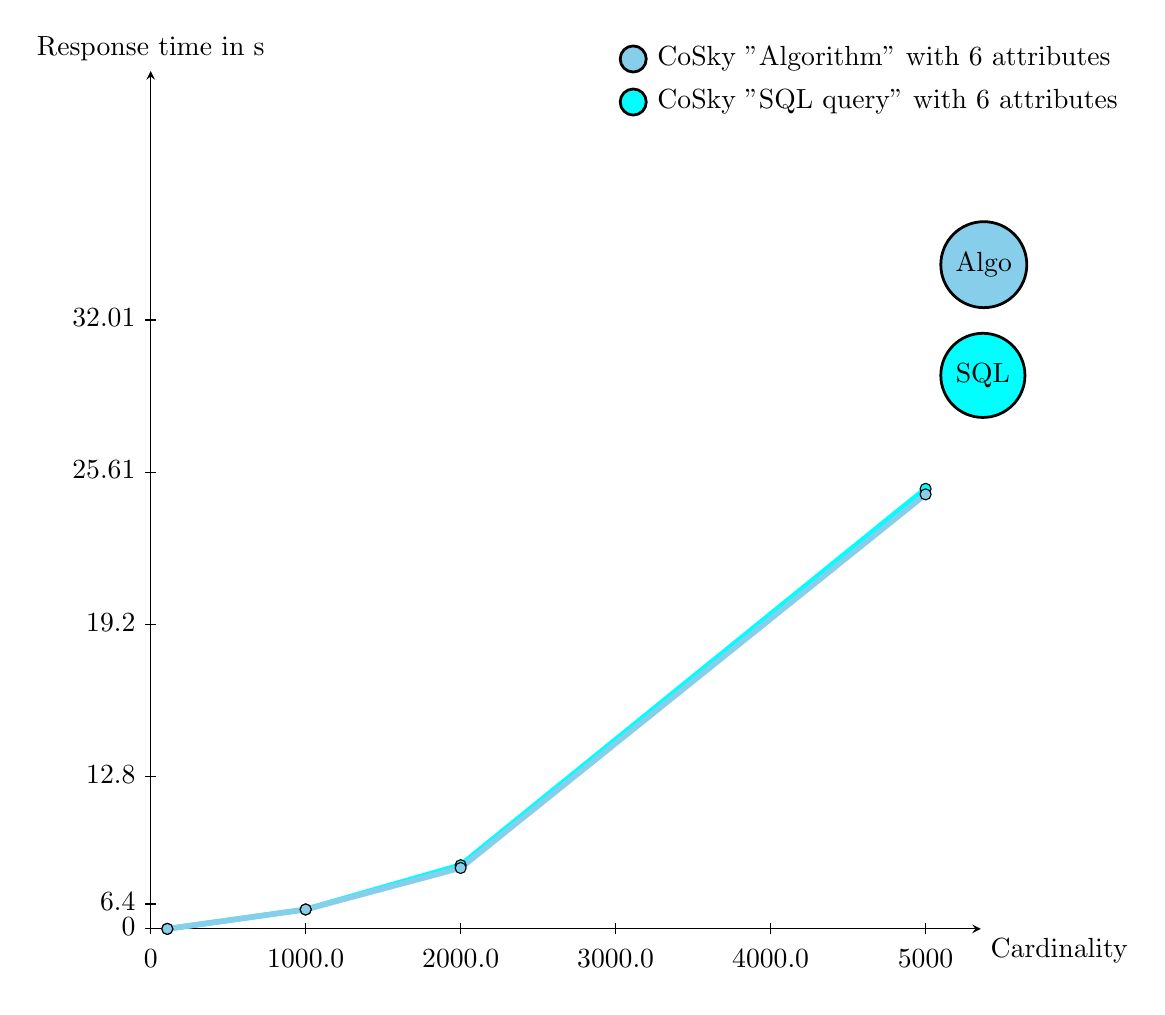
\begin{tikzpicture}[
                line join=bevel,
                bigcyannode/.style={shape=circle, fill=cyan, draw=black, line width=1pt},
                bigskybluenode/.style={shape=circle, fill=skyblue, draw=black, line width=1pt}
                ]
                %% Draws
                \draw[-stealth] (0pt, 0pt) -- (300pt, 0pt) node[anchor=north west] {Cardinality};
                \draw[-stealth] (0pt, 0pt) -- (0pt, 310pt) node[anchor=south] {Response time in s};

                        % Axis Graduation
                        \foreach \y/\ytext in {0pt/$0$, 9pt/$6.4$, 55pt/$12.8$, 110pt/$19.2$, 165pt/$25.61$, 220pt/$32.01$} {
                            \draw (2pt, \y) -- (-2pt, \y) node[left] {\ytext\strut};
                        }
            
                        \foreach \x/\xtext in {0pt/$0$, 56pt/$1000.0$, 112pt/$2000.0$, 168pt/$3000.0$, 224pt/$4000.0$, 280pt/$5000$} {
                            \draw (\x, 2pt) -- (\x, -2pt) node[below] {\xtext\strut};
                        }
                    
\draw[cyan, line width=2pt](6pt, 0pt) -- (56pt, 7pt) -- (112pt, 23pt) -- (280pt, 159pt);

\draw[skyblue, line width=2pt](6pt, 0pt) -- (56pt, 7pt) -- (112pt, 22pt) -- (280pt, 157pt);

\filldraw[color=black, fill=cyan] (6pt, 0pt) circle (2pt);
\filldraw[color=black, fill=cyan] (56pt, 7pt) circle (2pt);
\filldraw[color=black, fill=cyan] (112pt, 23pt) circle (2pt);
\filldraw[color=black, fill=cyan] (280pt, 159pt) circle (2pt);

\filldraw[color=black, fill=skyblue] (6pt, 0pt) circle (2pt);
\filldraw[color=black, fill=skyblue] (56pt, 7pt) circle (2pt);
\filldraw[color=black, fill=skyblue] (112pt, 22pt) circle (2pt);
\filldraw[color=black, fill=skyblue] (280pt, 157pt) circle (2pt);


                %% Caption
                \matrix [below left] at (current bounding box.north east) {
                \node [bigskybluenode, label=right:CoSky "Algorithm" with 6 attributes] {}; \\
                \node [bigcyannode, label=right:CoSky "SQL query" with 6 attributes] {}; \\
                };
                
                    \node[bigskybluenode, right=5pt] at (280pt,240pt) {Algo};
                    \node[bigcyannode, right=5pt] at (280pt,200pt) {SQL};
                    \end{tikzpicture}
                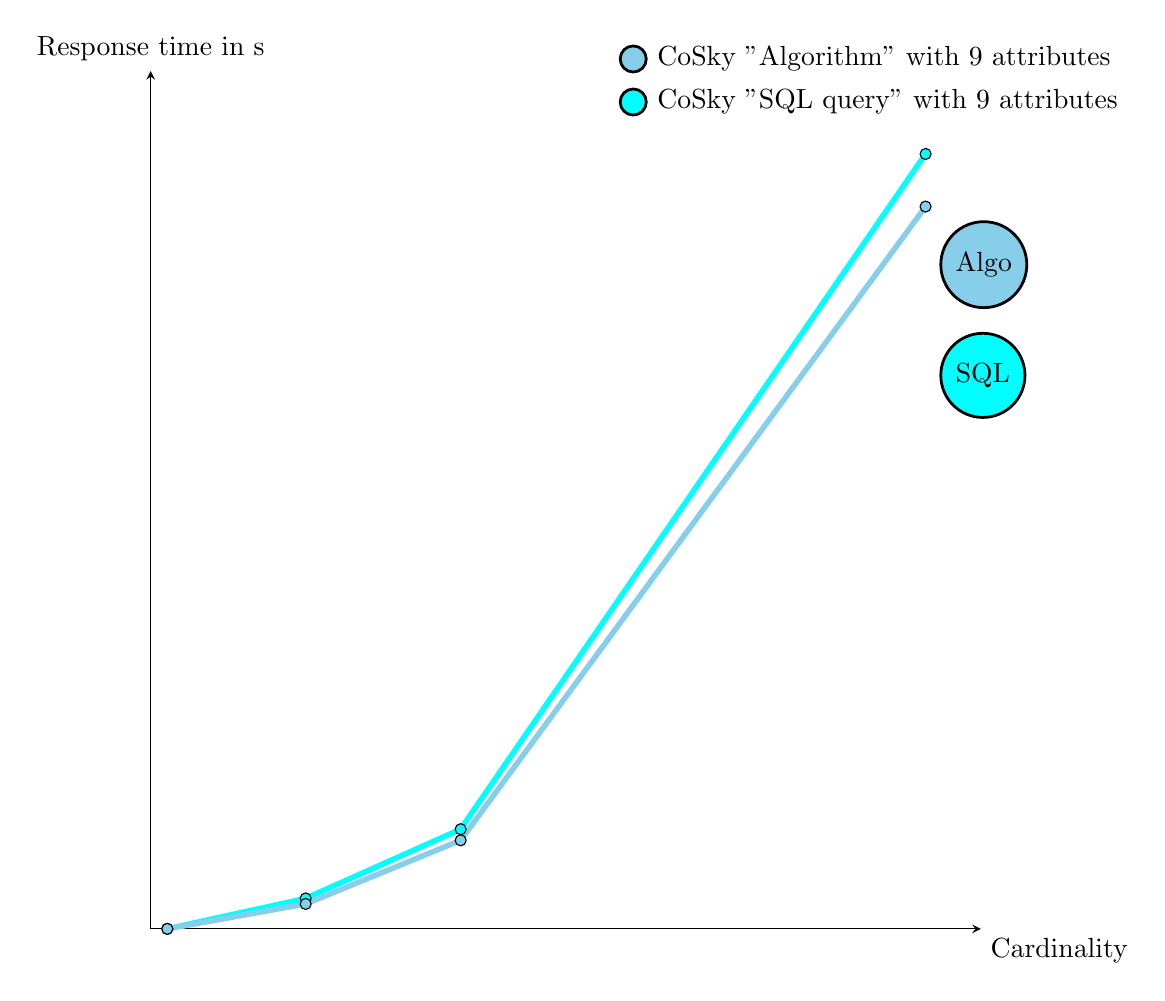
\begin{tikzpicture}[
                line join=bevel,
                bigcyannode/.style={shape=circle, fill=cyan, draw=black, line width=1pt},
                bigskybluenode/.style={shape=circle, fill=skyblue, draw=black, line width=1pt}
                ]
                %% Draws
                \draw[-stealth] (0pt, 0pt) -- (300pt, 0pt) node[anchor=north west] {Cardinality};
                \draw[-stealth] (0pt, 0pt) -- (0pt, 310pt) node[anchor=south] {Response time in s};

                        % Axis Graduation
                        
\draw[cyan, line width=2pt](6pt, 0pt) -- (56pt, 11pt) -- (112pt, 36pt) -- (280pt, 280pt);

\draw[skyblue, line width=2pt](6pt, 0pt) -- (56pt, 9pt) -- (112pt, 32pt) -- (280pt, 261pt);

\filldraw[color=black, fill=cyan] (6pt, 0pt) circle (2pt);
\filldraw[color=black, fill=cyan] (56pt, 11pt) circle (2pt);
\filldraw[color=black, fill=cyan] (112pt, 36pt) circle (2pt);
\filldraw[color=black, fill=cyan] (280pt, 280pt) circle (2pt);

\filldraw[color=black, fill=skyblue] (6pt, 0pt) circle (2pt);
\filldraw[color=black, fill=skyblue] (56pt, 9pt) circle (2pt);
\filldraw[color=black, fill=skyblue] (112pt, 32pt) circle (2pt);
\filldraw[color=black, fill=skyblue] (280pt, 261pt) circle (2pt);

%% Caption
			    \matrix [below left] at (current bounding box.north east) {
				\node [bigskybluenode, label=right:CoSky "Algorithm" with 9 attributes] {}; \\
				\node [bigcyannode, label=right:CoSky "SQL query" with 9 attributes] {}; \\
			    };
                    \node[bigskybluenode, right=5pt] at (280pt,240pt) {Algo};
                    \node[bigcyannode, right=5pt] at (280pt,200pt) {SQL};
                    \end{tikzpicture}
                    \end{document}